\section{Results}
\label{sec:results}

The data-driven probabilistic model we have presented produces good-looking patterns and can be applied to a variety of tasks. The factor graph representation makes it easy to adapt our framework to handle new problems or incorporate user-provided design constraints by introducing additional factors to the factor graph, or changing the source data used to train the factor weights and histograms.

\remark{Discuss parameters used to train model ``unless otherwise specified''. Number of artists, weights, etc.}

\remark{Describe how we use the Colourlovers site to render the final images.}

\subsection{Coloring Pattern Templates}

\begin{figure*}[ht]
\begin{tabular}{ccc}

\includegraphics[width=.15\linewidth]{figs/permutationTemplatePalette} & 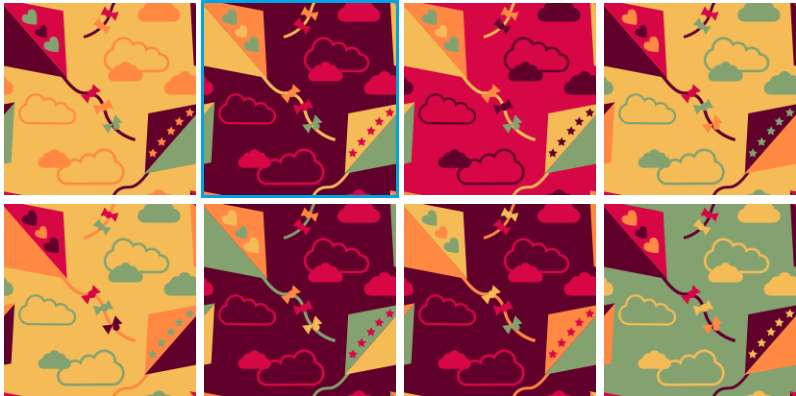
\includegraphics[width=.4\linewidth]{figs/permutationBest8} & 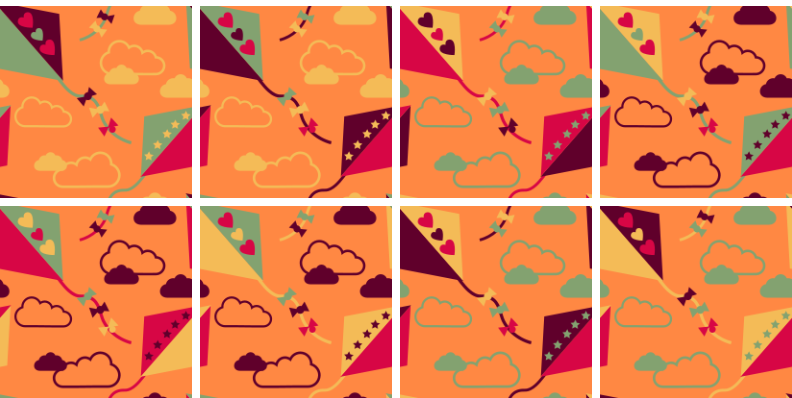
\includegraphics[width=.4\linewidth]{figs/permutationWorst8} %& 
\includegraphics[width=.12\linewidth]{figs/permutationArtist}
  \\
\textbf{(a)} Input Pattern & \textbf{(b)} Highest-scoring assignments & \textbf{(c)} Lowest-scoring assignments %& \textbf{(d)} Artist assignment
\\
\end{tabular}

\caption{Given a segmented image and corresponding palette as input, we use our color model to compute the likelihood of each possible assignment of the palette to the image regions. \textbf{(b)} and \textbf{(c)} show the top-eight and bottom-eight assignments. The assignment provided by the artist received the second-highest score and is highlighted in blue.}
\label{fig:permutation}
\end{figure*}

\paragraph{Spatial arrangement} In some cases, an artist already knows what colors they want to use in an image. They might have found a palette they are enamored with elsewhere, or they might have a very specific theme in mind. Even with a fixed palette, there are still a range of images that can be created by mapping different colors to different regions, only some of which are desirable to the artist. To support this task, we rank all 120 possible permutations of the colors using the score assigned by our model.~\remark{D: This assumes a 5-color-group pattern.} Figure~\ref{fig:permutation} shows one example of this process. \ref{fig:permutation}b shows the eight highest-rated color assignments which exhibits a variety of color styles and contrasts strongly against the lowest-rated assignments. Our color model assignment a very low score to assigning the tangerine color to the background region because its color properties were not similar to background colors in the model's training set. The actual color assignment originally provided by the artist for this color template received the second-highest score, suggesting that our model was able to capture the artist's intent.

\begin{figure}[ht]
\begin{tabular}{cc}
\raisebox{2em}{
\includegraphics[width=.22\columnwidth]{figs/guidedSearch0Original}}&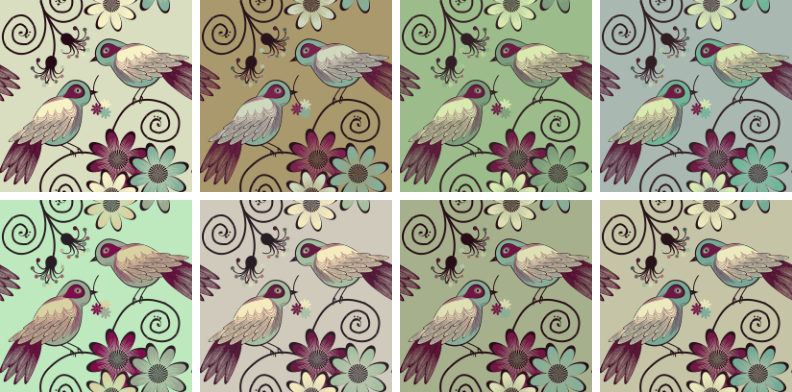
\includegraphics[width=.7\columnwidth]{figs/guidedSearch0MMR}\vspace{0.5em}\\
\raisebox{2em}{
\includegraphics[width=.22\columnwidth]{figs/guidedSearch1Original}}&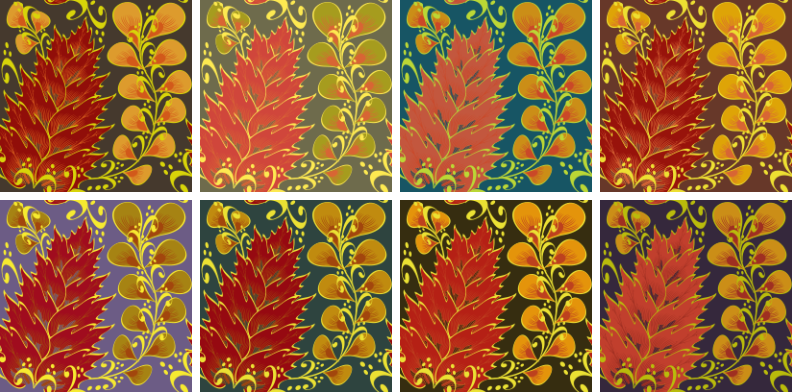
\includegraphics[width=.7\columnwidth]{figs/guidedSearch1MMR}\vspace{0.5em}\\
\raisebox{2em}{
\includegraphics[width=.22\columnwidth]{figs/guidedSearch2Original}}&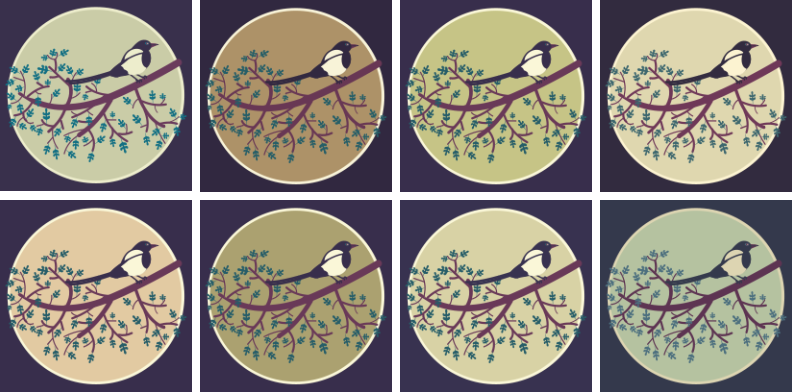
\includegraphics[width=.7\columnwidth]{figs/guidedSearch2MMR}\\
Suggestion&Results\\
\end{tabular}

\caption{An artist provides an initial color assignment and asks for patterns that are similar. We incorporate this request by adding an additional factor to our model, showing eight samples drawn from the new model for each of the suggested images.}
\label{fig:nearbySuggestions}
\vspace{-1.0em}
\end{figure}

\begin{figure}[ht]
\begin{tabular}{ccc} 
Style&Example&Results\\ %\hline
\raisebox{1.55em}{\emph{Light}}&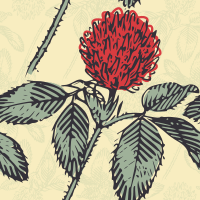
\includegraphics[width=.148\columnwidth]{figs/styleResultsLightExample}&
\includegraphics[width=.62\columnwidth]{figs/styleResultsLight}\vspace{0.5em}\\
\raisebox{1.55em}{\emph{Dark}}&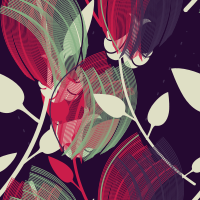
\includegraphics[width=.148\columnwidth]{figs/styleResultsDarkExample}&
\includegraphics[width=.62\columnwidth]{figs/styleResultsDark}\vspace{0.5em}\\
\raisebox{1.55em}{\emph{Bold}}&
\includegraphics[width=.148\columnwidth]{figs/styleResultsBoldExample}&
\includegraphics[width=.62\columnwidth]{figs/styleResultsBold}\vspace{0.5em}\\
\raisebox{1.55em}{\emph{Mellow}}&
\includegraphics[width=.148\columnwidth]{figs/styleResultsMellowExample}&
\includegraphics[width=.62\columnwidth]{figs/styleResultsMellow}\vspace{0.5em}\\
\end{tabular}

\caption{In this example, 17 patterns were chosen in three different styles, and a representative image from each style is shown in the second column. A separate model was then trained on each style, and in the third column we show four samples drawn from each model. In each case, our model is able to learn different properties of the desired distribution over colors.}
\label{fig:styleTraining}
\vspace{-1.0em}
\end{figure}

\begin{figure*}[ht]
\begin{tabular}{cc} 
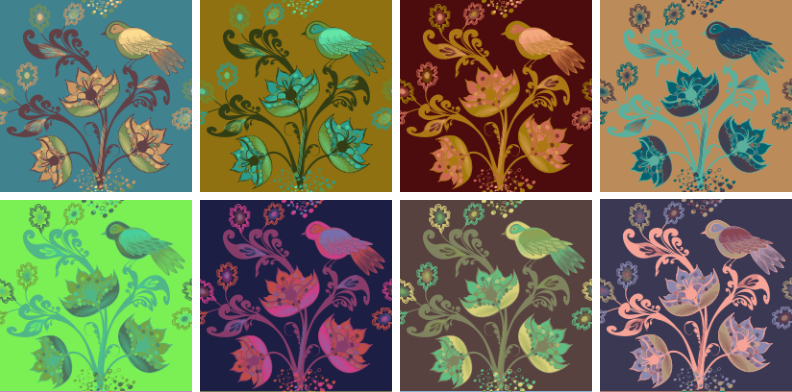
\includegraphics[width=.475\linewidth]{figs/constrainedSearchUnconstrained}&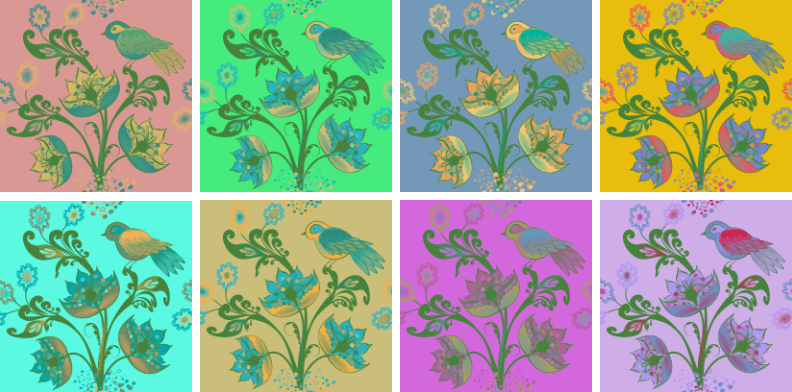
\includegraphics[width=.475\linewidth]{figs/constrainedSearchConstrained}\\
Unconstrained sampling&Constrained sampling\\
\end{tabular}

\caption{An artist coloring a pattern is presented with the results shown on the left, and decides that she only likes results where the stem of the plant is dark green. On the right, we use conditional inference to sample from our model subject to the constraint that the desired palette entry is fixed to a specific color. This is a natural way to incorporate semantic information about region colors which cannot be easily learned by our model.}
\label{fig:constrainedInference}
\vspace{-1.0em}
\end{figure*}

\begin{figure*}[ht]
\begin{tabular}{cc} 
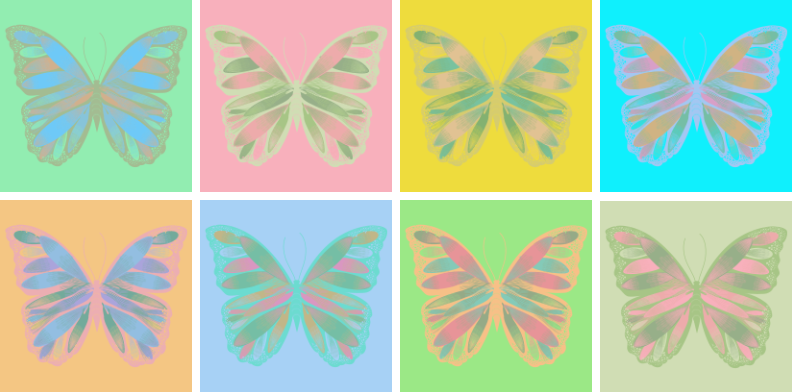
\includegraphics[width=.475\linewidth]{figs/styleSugar}&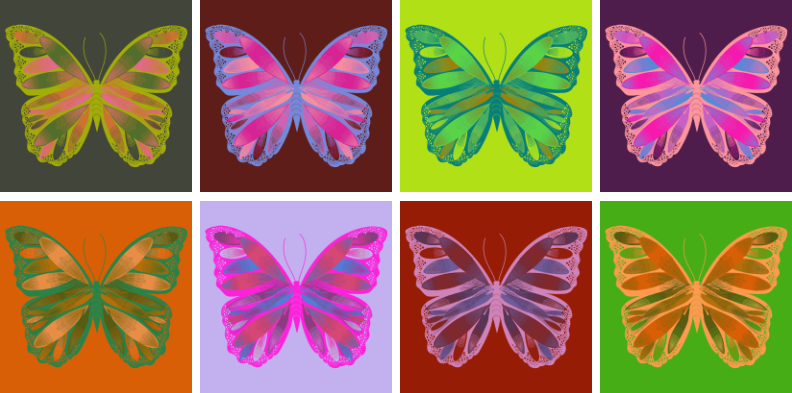
\includegraphics[width=.475\linewidth]{figs/styleAlbenaj}\\
Artist A&Artist B\\
\end{tabular}

\caption{Our data-driven approach makes it easy to capture the styles of different artists. Here, we show results sampled from two different models, each trained on 100 images of a single artist.}
\vspace{-1.0em}
\end{figure*}

\subsection{Performance}

Performance figures? (training time, inference time, etc.)